
\begin{center}\rule{0.5\linewidth}{0.5pt}\end{center}

\section{ЧАСТЬ 1: Руководство администратора}\label{KT-3.1_User_Guide-ux447ux430ux441ux442ux44c-1-ux440ux443ux43aux43eux432ux43eux434ux441ux442ux432ux43e-ux430ux434ux43cux438ux43dux438ux441ux442ux440ux430ux442ux43eux440ux430}

\subsection{Системные требования}\label{KT-3.1_User_Guide-ux441ux438ux441ux442ux435ux43cux43dux44bux435-ux442ux440ux435ux431ux43eux432ux430ux43dux438ux44f}

\begin{longtable}[]{@{}lll@{}}
\toprule\noalign{}
Компонент & Минимум & Рекомендуется \\
\midrule\noalign{}
\endhead
\bottomrule\noalign{}
\endlastfoot
ОС & Windows 10 / Ubuntu 20.04 & Windows 11 / Ubuntu 24.04 \\
Компилятор & Clang 22 (или clang-cl 22 для Windows) & --- \\
CMake & 3.30+ & --- \\
Бэкенд сборки & Ninja 1.13+ & --- \\
Vulkan SDK & 1.4.350+ & --- \\
GPU & Поддержка Vulkan 1.4 & Дискретная GPU с 4+ GB VRAM \\
ОЗУ & 8 GB & 16 GB \\
Диск & 5 GB (исходники + build + assets) & 10 GB SSD \\
\end{longtable}

\textbf{Сетевые порты:} не требуются (приложение однопроцессное, не открывает портов).

\subsection{Инструкция по развёртыванию (Linux)}\label{KT-3.1_User_Guide-ux438ux43dux441ux442ux440ux443ux43aux446ux438ux44f-ux43fux43e-ux440ux430ux437ux432ux451ux440ux442ux44bux432ux430ux43dux438ux44e-linux}

\begin{verbatim}
# 1. Клонирование репозитория с подмодулями
git clone --recursive https://github.com/Leeleit/ProjectV.git
cd ProjectV

# 2. Конфигурация CMake (preset linux-clang-debug)
cmake --preset linux-clang-debug
#    → создаст build/linux-clang-debug/ с Ninja-конфигурацией

# 3. Сборка (~ 5–15 минут на 16 ядрах)
cmake --build build/linux-clang-debug --parallel

# 4. Запуск runtime-смоук-теста
./tools/linux/Invoke-ProjectVRuntimeSmoke.sh
#    → генерирует 6 captures (FINAL, SHDW, CSM, CTSH, AOCC, LOCL)
#    → в build/linux-clang-debug/lookdev-captures/

# 5. Запуск приложения напрямую
./build/linux-clang-debug/src/app/ProjectV
\end{verbatim}

\subsection{Инструкция по развёртыванию (Windows)}\label{KT-3.1_User_Guide-ux438ux43dux441ux442ux440ux443ux43aux446ux438ux44f-ux43fux43e-ux440ux430ux437ux432ux451ux440ux442ux44bux432ux430ux43dux438ux44e-windows}

\begin{verbatim}
# 1. Клонирование
git clone --recursive https://github.com/Leeleit/ProjectV.git
cd ProjectV

# 2. Конфигурация (preset windows-clang-debug)
cmake --preset windows-clang-debug

# 3. Сборка (clang-cl + Ninja)
cmake --build build/windows-clang-debug --parallel

# 4. Запуск runtime-смоук-теста
powershell -ExecutionPolicy Bypass -File tools\windows\Invoke-ProjectVRuntimeSmoke.ps1
#    → генерирует 6 captures (FINAL, SHDW, CSM, CTSH, AOCC, LOCL)
#    → в build\windows-clang-debug\lookdev-captures\

# 5. Запуск приложения напрямую
build\windows-clang-debug\src\app\ProjectV.exe
\end{verbatim}

\subsection{Переменные окружения}\label{KT-3.1_User_Guide-ux43fux435ux440ux435ux43cux435ux43dux43dux44bux435-ux43eux43aux440ux443ux436ux435ux43dux438ux44f}

\begin{longtable}[]{@{}lll@{}}
\toprule\noalign{}
Имя & Назначение & Значение по умолчанию \\
\midrule\noalign{}
\endhead
\bottomrule\noalign{}
\endlastfoot
\texttt{VULKAN\_SDK} & Путь к Vulkan SDK (для шейдеров и валидации) & автоопределение CMake \\
\texttt{PROJECTV\_ENABLE\_VALIDATION} & Включить Vulkan validation layers & \texttt{ON} (debug), \texttt{OFF} (release) \\
\texttt{PROJECTV\_RENDERER\_DEBUG} & Поднять дебаг-HUD (FPS, draw calls, frame time) & \texttt{OFF} \\
\texttt{PROJECTV\_ASSET\_DIR} & Каталог с glTF-ассетами & \texttt{assets/} \\
\texttt{PROJECTV\_SCENE\_PRESET} & Пресет сцены при старте & \texttt{VoxelLab} \\
\texttt{VK\_INSTANCE\_LAYERS} & Список Vulkan-слоёв (для отладки) & \texttt{VK\_LAYER\_KHRONOS\_validation} \\
\end{longtable}

\subsection{Пресеты сцен}\label{KT-3.1_User_Guide-ux43fux440ux435ux441ux435ux442ux44b-ux441ux446ux435ux43d}

ProjectV поставляется с пресетами сцен, демонстрирующими разные аспекты движка:

\begin{longtable}[]{@{}ll@{}}
\toprule\noalign{}
Пресет & Назначение \\
\midrule\noalign{}
\endhead
\bottomrule\noalign{}
\endlastfoot
\texttt{VoxelLab} & Базовая сцена с оболочкой, opaque-anchor\textquotesingle ами и fluid-зоной \\
\texttt{FlatBenchmark} & Плоская платформа 64×64 без объектов --- baseline для тени/мешинга \\
\texttt{TransparencyStress} & Сетка стеклянных столбов 2×2, высота 4--12 --- нагрузка на alpha-blending \\
\texttt{ChunkGrid} & Вертикальные столбы на границах чанков --- лес для проверки длинных теней \\
\texttt{MeshingStress} & Объём из вокселей в шахматном 3D-порядке --- стресс-тест greedy-мешинга \\
\end{longtable}

\textbf{Реализация в коде} (\texttt{src/voxel/VoxelWorld.cpp}):

\begin{itemize}
\tightlist
\item
  \texttt{VoxelLab} --- \texttt{BuildVoxelLabSceneWorld()} → \texttt{BuildVoxelLabShellAndFluid} + \texttt{BuildVoxelLabOpaqueAnchors}.
\item
  \texttt{FlatBenchmark} --- \texttt{BuildFlatBenchmarkSceneWorld()} (только \texttt{CreateSceneWorldWithFloor} + \texttt{BuildCheckerboardFloor}).
\item
  \texttt{TransparencyStress} --- \texttt{BuildTransparencyStressSceneWorld()} → \texttt{BuildTransparencyStressColumns} (стеклянные столбы в \texttt{BuildTransparencyStressColumns}, высоты 4--12 от \texttt{(x+z)\%8}).
\item
  \texttt{ChunkGrid} --- \texttt{BuildChunkGridSceneWorld()} → \texttt{BuildChunkGridMarkers} (столбы на каждой границе чанка, чередование FloorWhite/FloorGray по \texttt{(chunkX+chunkZ)\%2}).
\item
  \texttt{MeshingStress} --- \texttt{BuildMeshingStressSceneWorld()} → \texttt{BuildMeshingStressVolume} (объём через \texttt{(x+y+z)\%2}, чередование FloorWhite/FloorGray по \texttt{(x+z)\%2}, высота до 16).
\end{itemize}

Кроме того, в коде есть fluid-мешинг (\texttt{voxel\_fluid.comp} + \texttt{VoxelMaterial::Fluid=2}) --- он не выделен в отдельный пресет, но может быть включён через \texttt{PROJECTV\_SCENE\_PRESET} в любую сцену, если в её JSON указано использование \texttt{Fluid} материала.

\textbf{Скриншоты (VoxelLab и стресс-пресеты):}

\pandocbounded{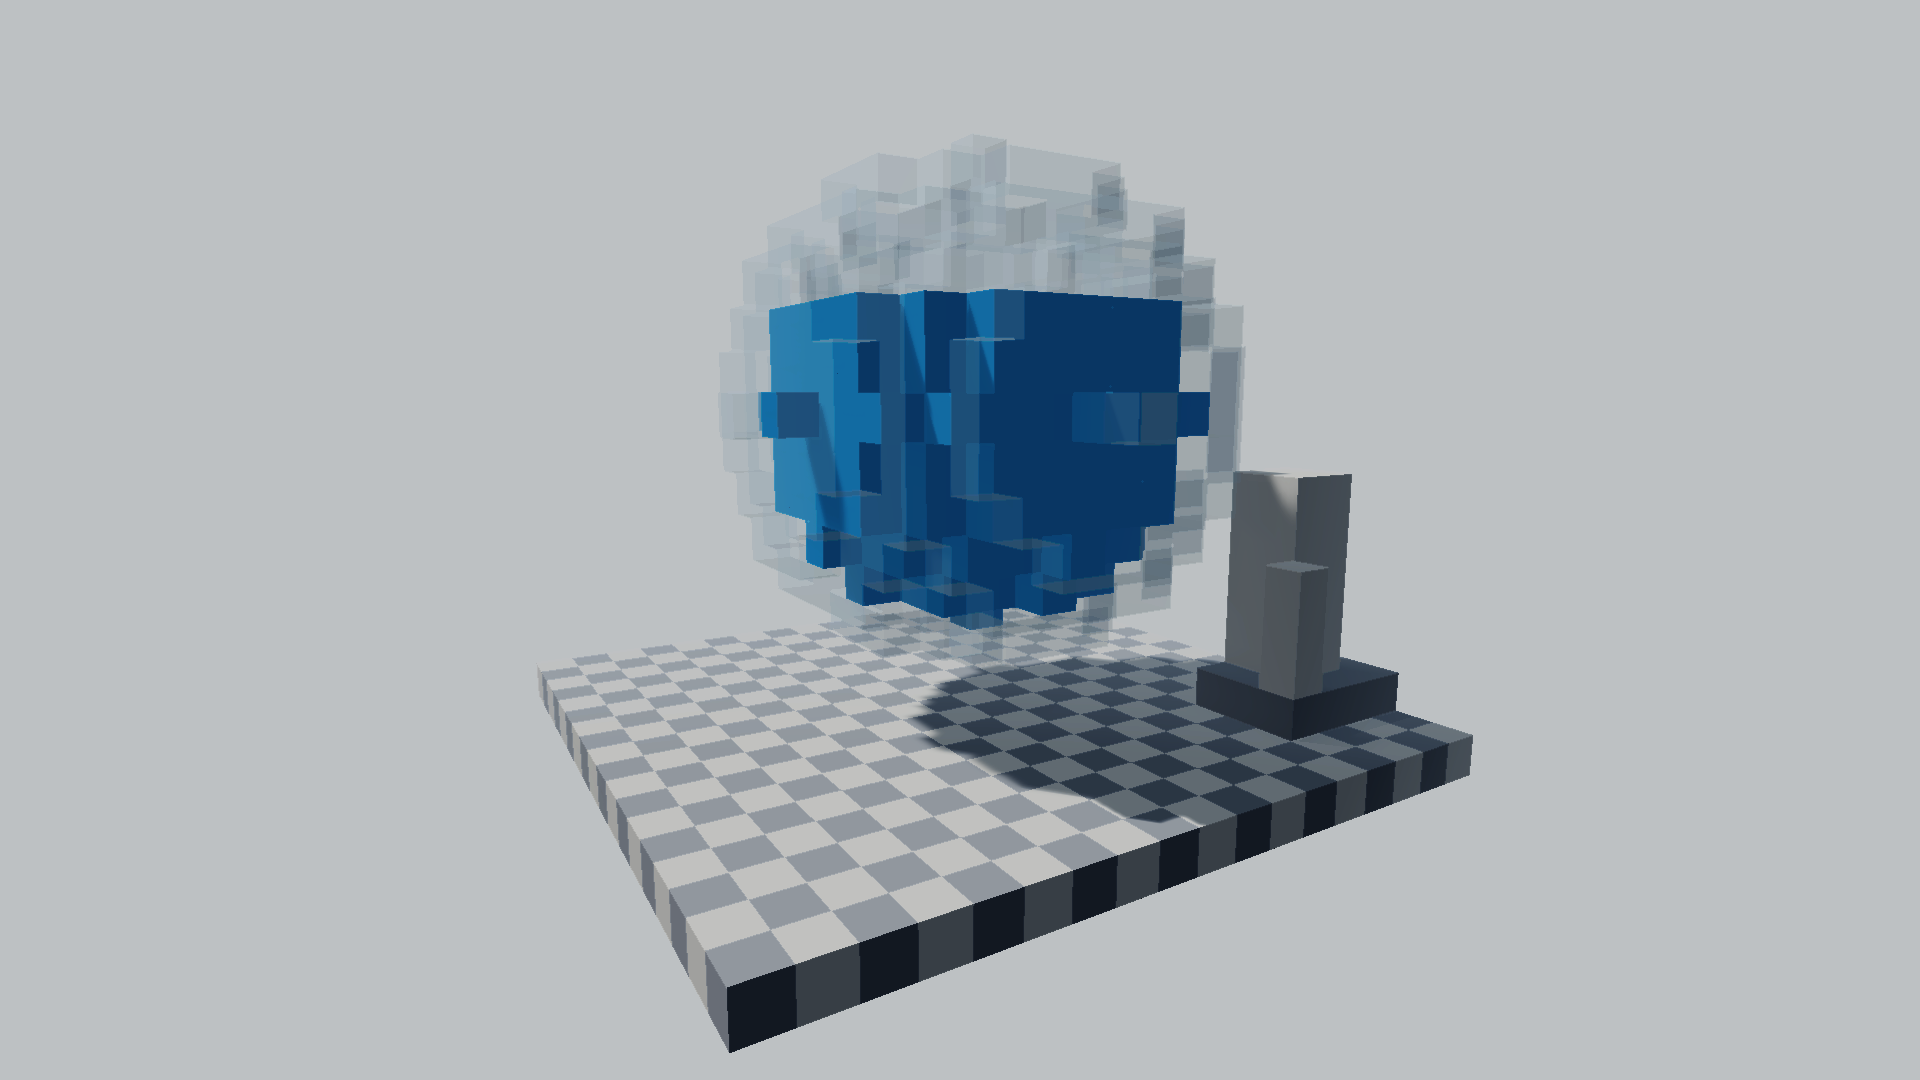
\includegraphics[keepaspectratio]{screenshots/kt-3.1/VoxelLab.png}}

\pandocbounded{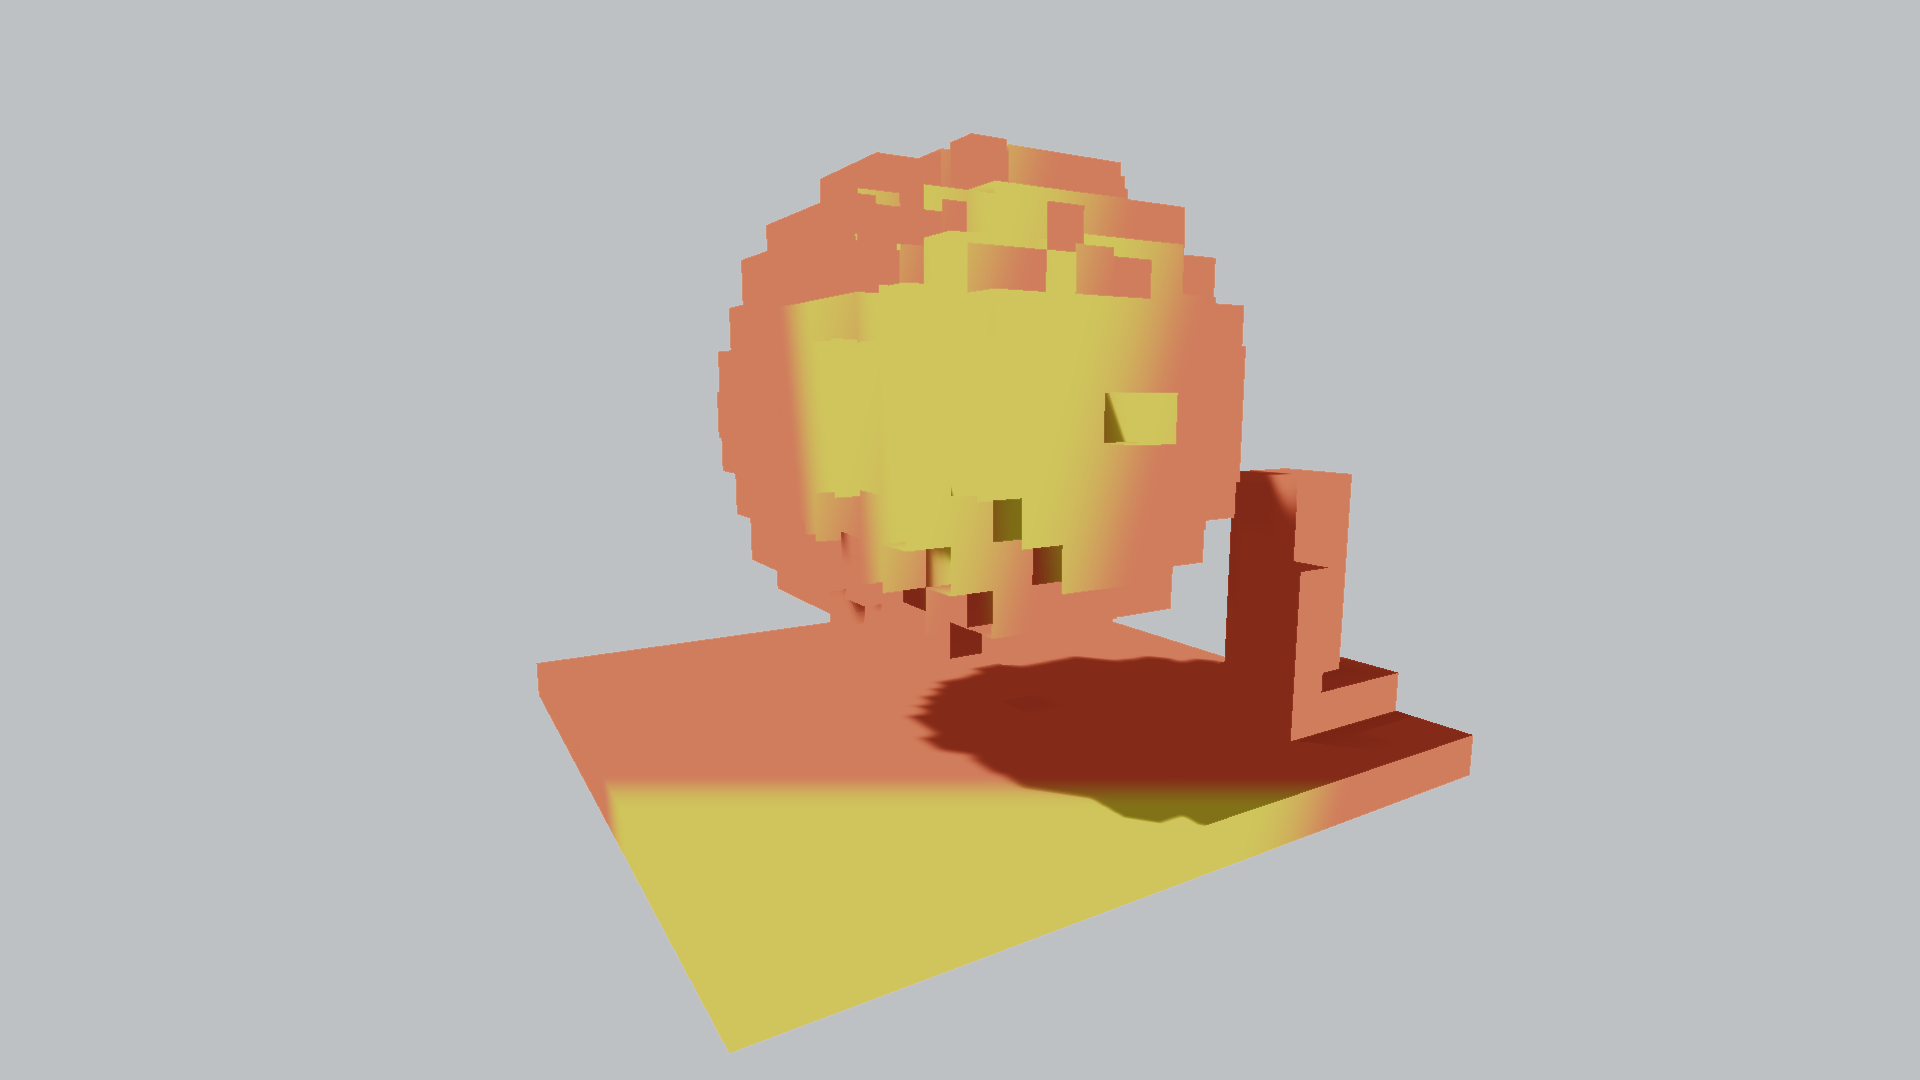
\includegraphics[keepaspectratio]{screenshots/kt-3.1/FlatBenchmark.png}}

\pandocbounded{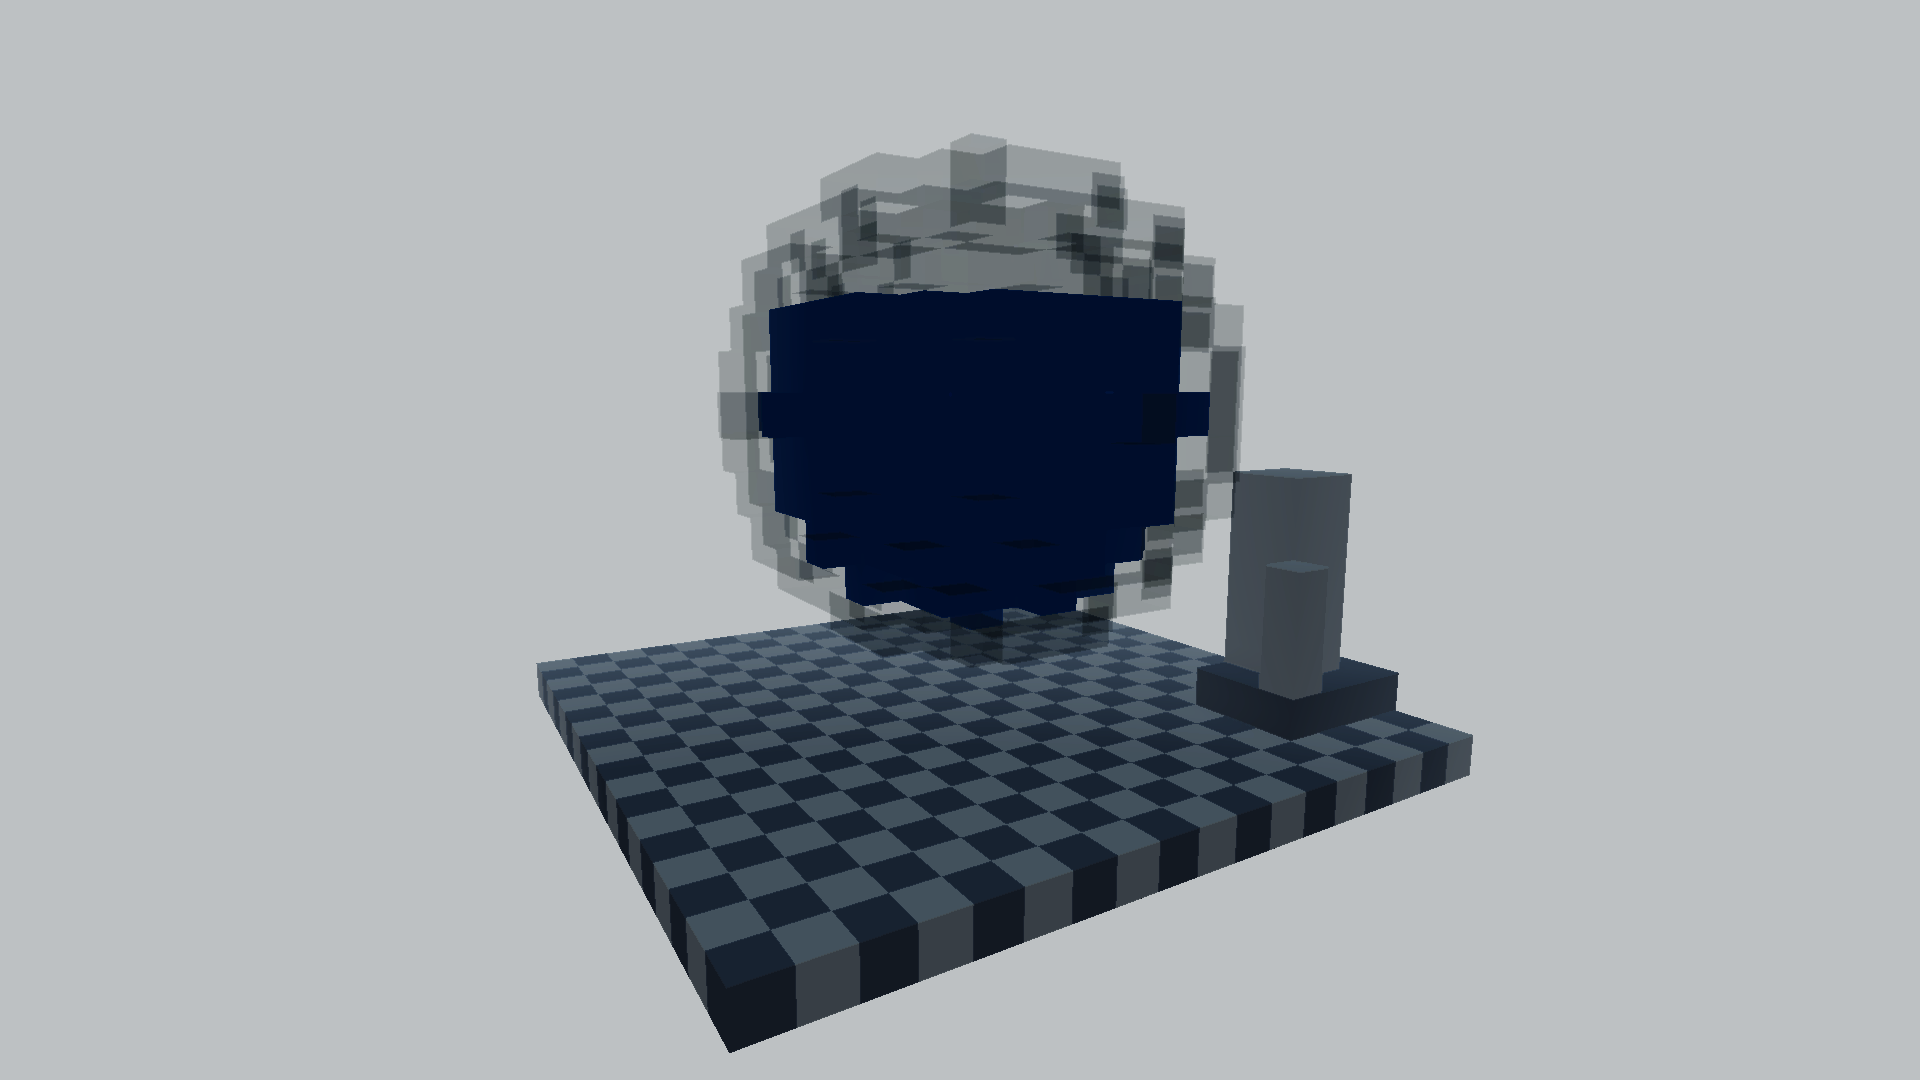
\includegraphics[keepaspectratio]{screenshots/kt-3.1/TransparencyStress.png}}

\pandocbounded{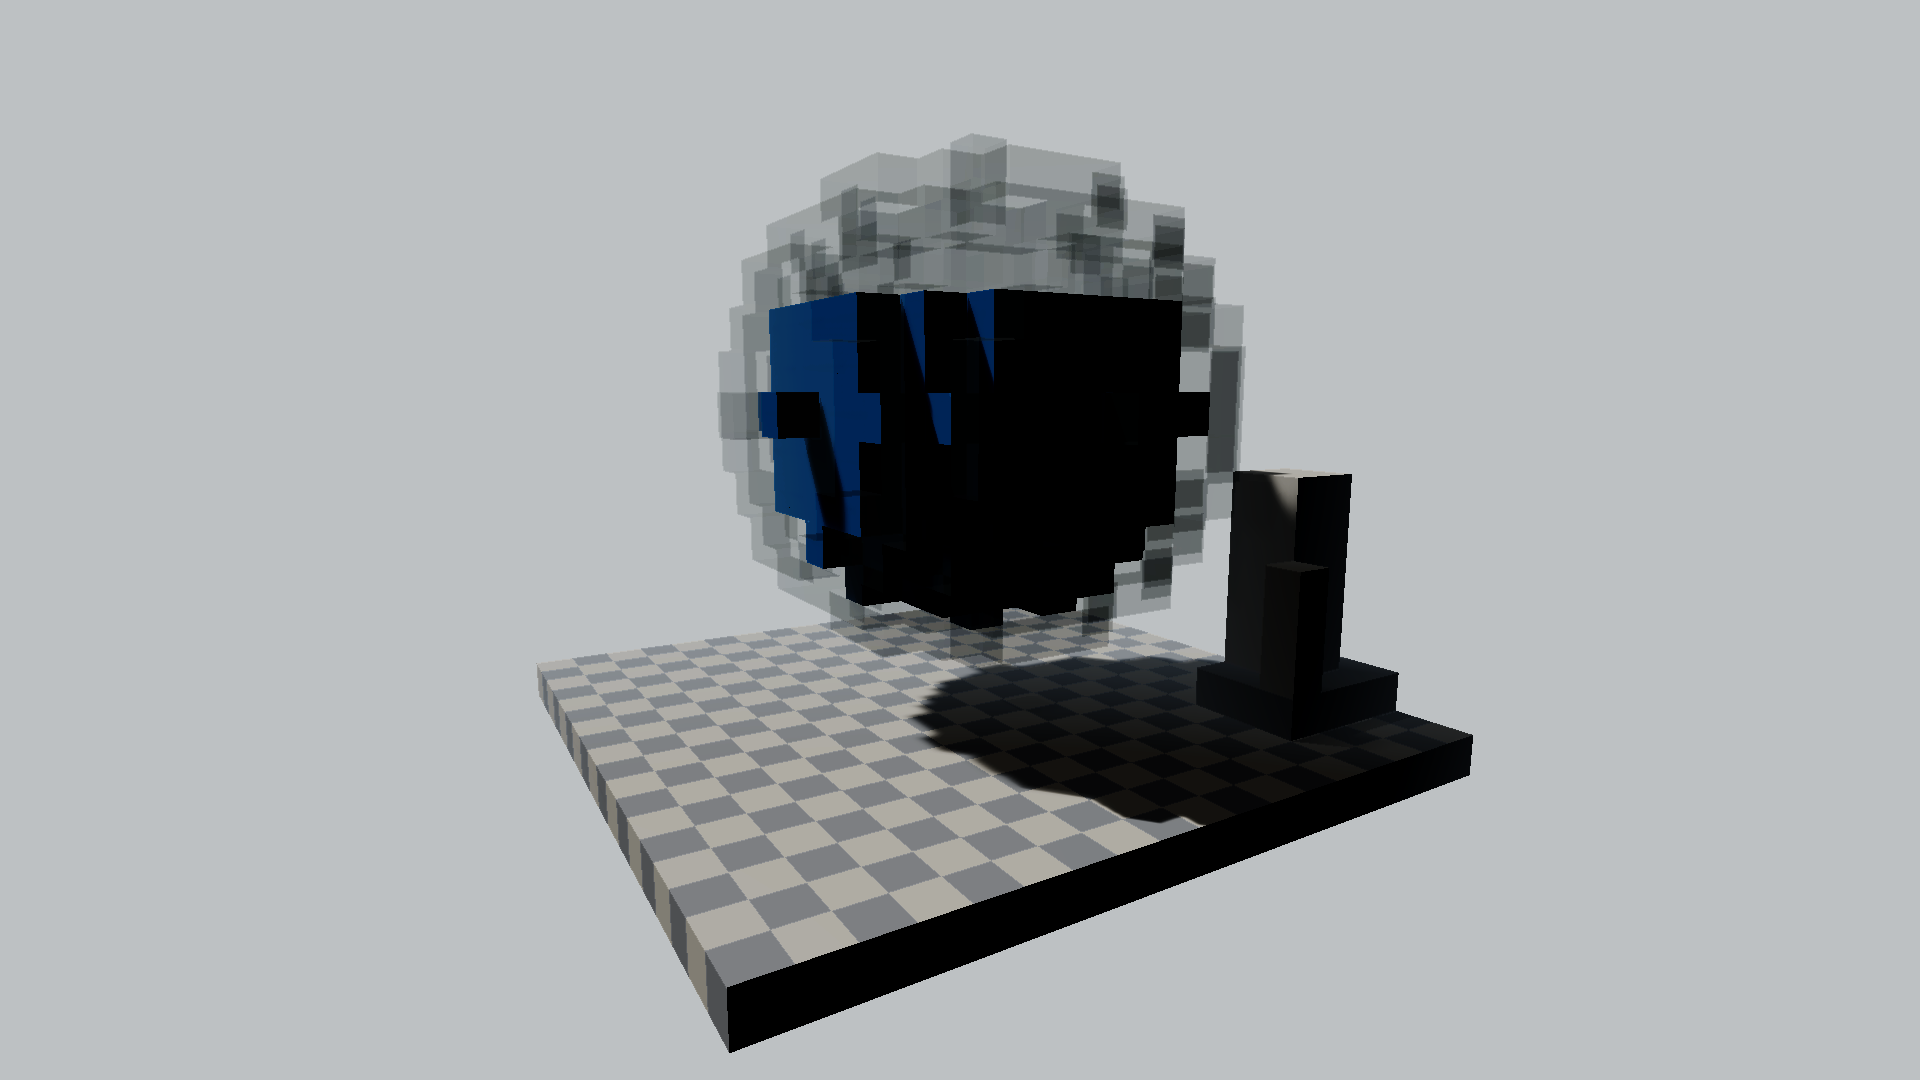
\includegraphics[keepaspectratio]{screenshots/kt-3.1/MeshingStress.png}}

\pandocbounded{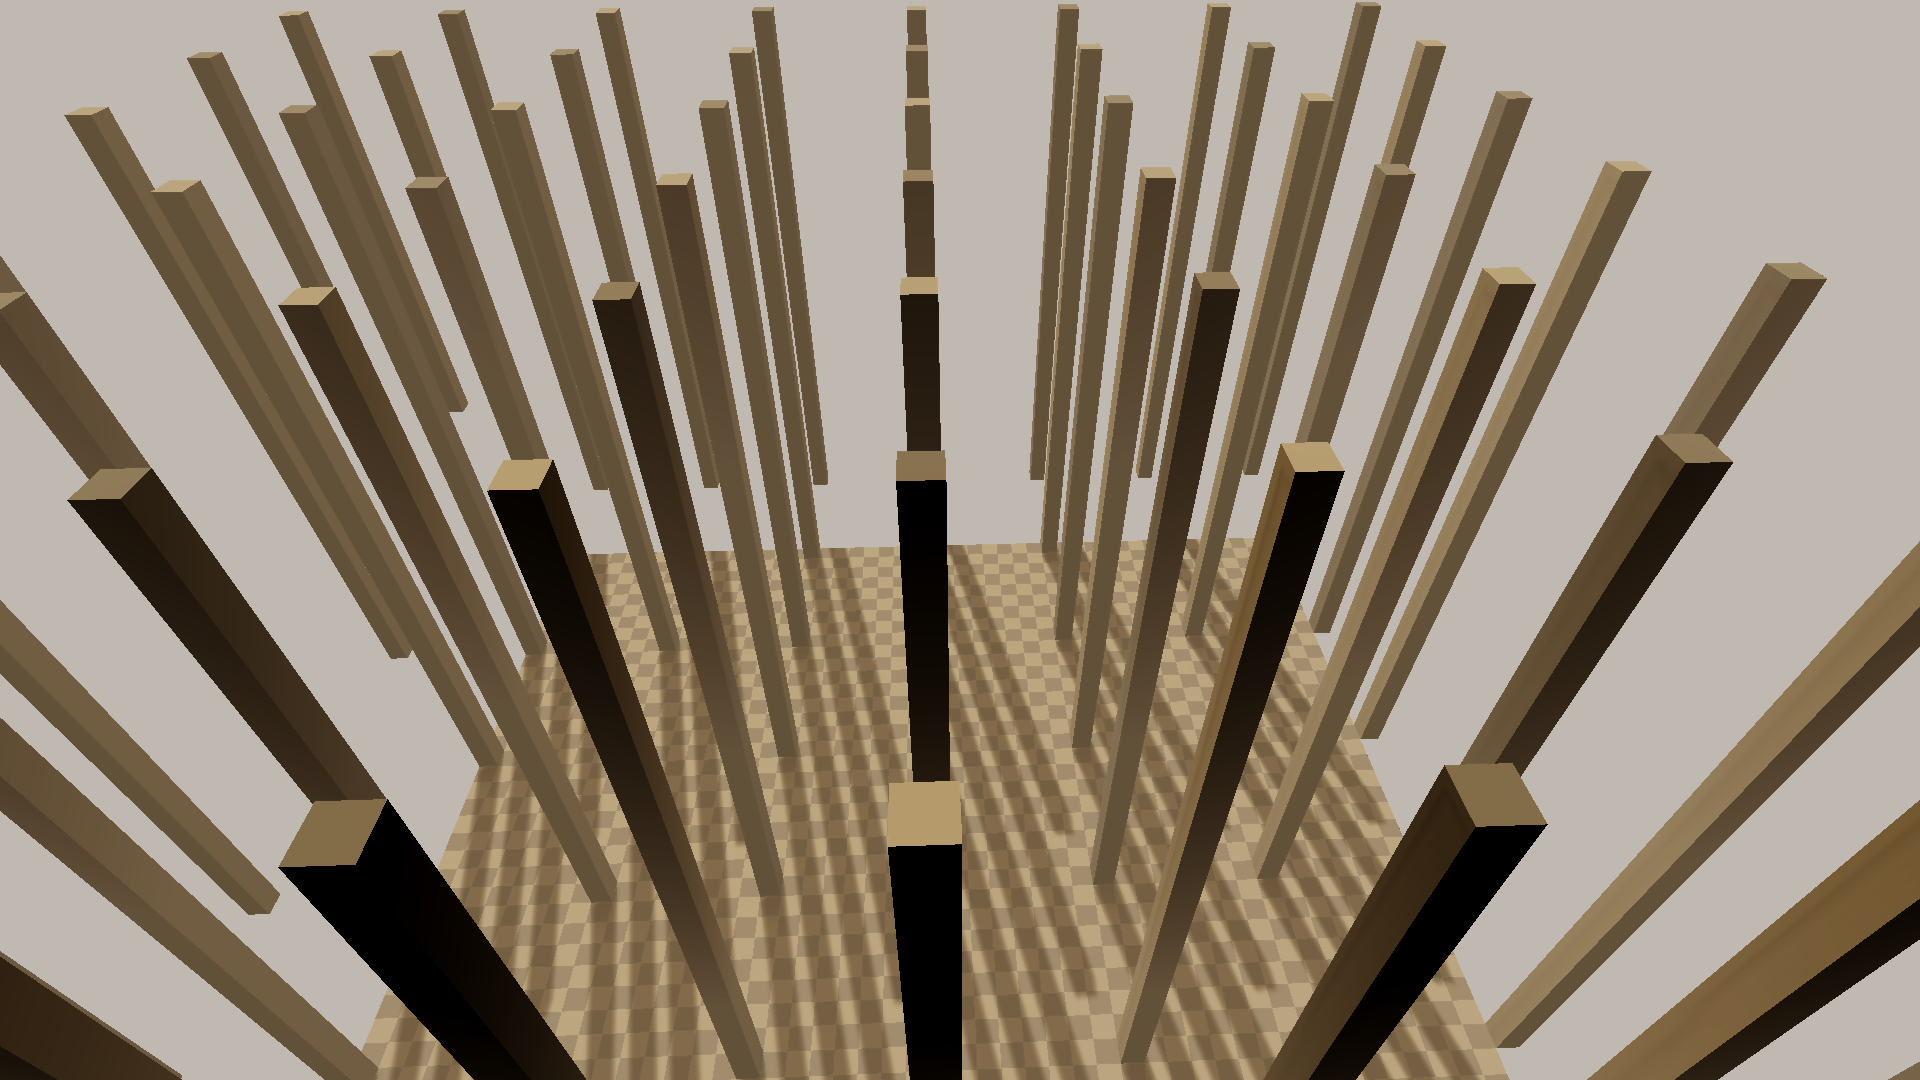
\includegraphics[keepaspectratio]{screenshots/kt-3.1/ChunkGrid.png}}

\pandocbounded{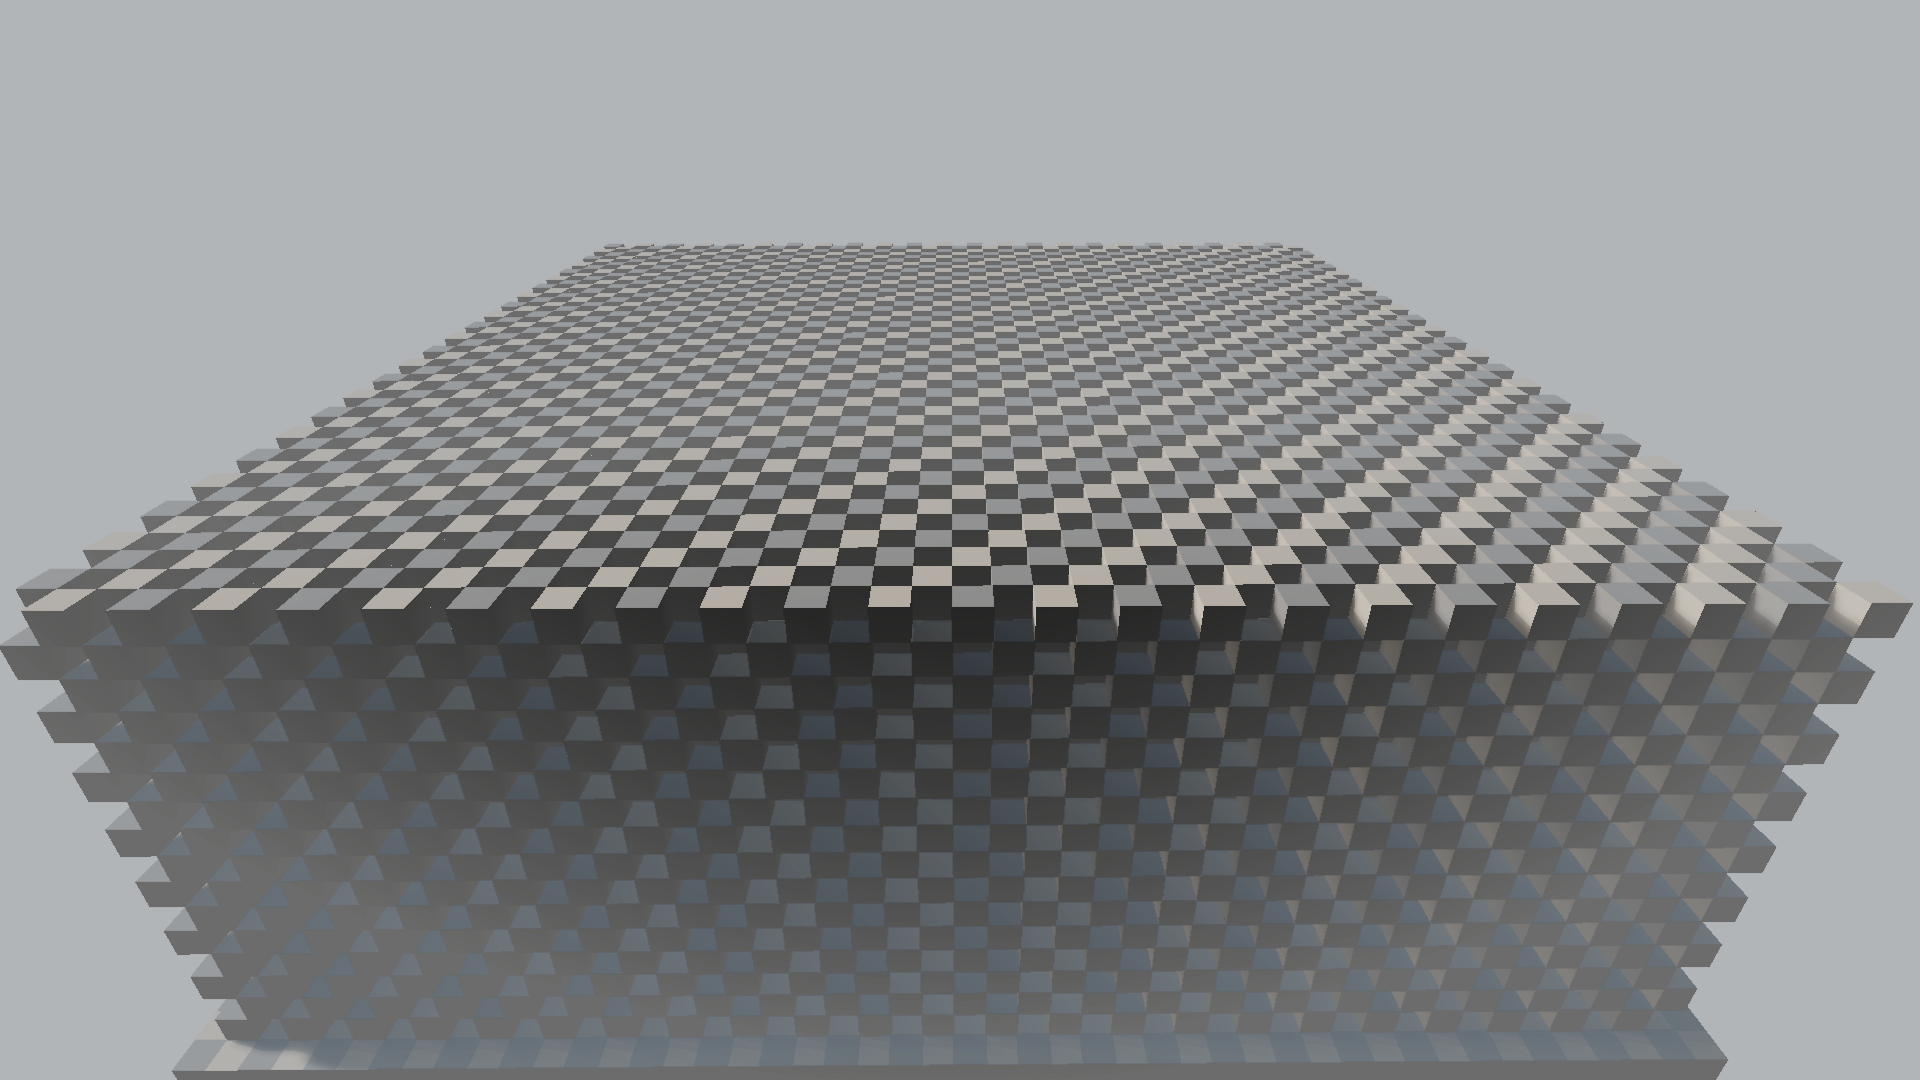
\includegraphics[keepaspectratio]{screenshots/kt-3.1/FluidDemo.png}}

\begin{center}\rule{0.5\linewidth}{0.5pt}\end{center}

\section{ЧАСТЬ 2: Руководство пользователя}\label{KT-3.1_User_Guide-ux447ux430ux441ux442ux44c-2-ux440ux443ux43aux43eux432ux43eux434ux441ux442ux432ux43e-ux43fux43eux43bux44cux437ux43eux432ux430ux442ux435ux43bux44f}

\subsection{Обзор интерфейса}\label{KT-3.1_User_Guide-ux43eux431ux437ux43eux440-ux438ux43dux442ux435ux440ux444ux435ux439ux441ux430}

Графическое окно \texttt{ProjectV} --- single-window desktop-приложение. Основные элементы:

\begin{longtable}[]{@{}lll@{}}
\toprule\noalign{}
\# & Элемент & Описание \\
\midrule\noalign{}
\endhead
\bottomrule\noalign{}
\endlastfoot
1 & Главный viewport & Рендер сцены с активной камерой (WASD + мышь) \\
2 & Debug HUD (опц.) & FPS, draw calls, frame time (вкл. \texttt{G}) \\
\end{longtable}

\subsection{Управление}\label{KT-3.1_User_Guide-ux443ux43fux440ux430ux432ux43bux435ux43dux438ux435}

Полный список кнопок --- в \texttt{src/app/InputActions.cpp} (\texttt{BindAction} вызовы). Ниже --- основные.

\begin{longtable}[]{@{}ll@{}}
\toprule\noalign{}
Клавиша & Действие \\
\midrule\noalign{}
\endhead
\bottomrule\noalign{}
\endlastfoot
\texttt{W} / \texttt{S} / \texttt{A} / \texttt{D} & Движение камеры (вперёд / назад / влево / вправо) \\
\texttt{Space} & Подъём камеры \\
\texttt{LShift} / \texttt{RShift} & Спуск камеры \\
\texttt{LCtrl} / \texttt{RCtrl} & Ускорение движения \\
\texttt{LAlt} / \texttt{RAlt} & Замедление движения \\
\texttt{ЛКМ} (mouse) & Удалить воксель под курсором (raycast) \\
\texttt{ПКМ} (mouse) & Разместить воксель под курсором (raycast) \\
\texttt{Tab} & Переключить relative mouse mode (для FPS-управления) \\
\texttt{F1} & Toggle HUD (показать/скрыть) \\
\texttt{F2} & Cycle placement material (Air/Glass/Fluid/FloorWhite/FloorGray) \\
\texttt{F3} & Reset camera (вернуть в начальную позицию) \\
\texttt{F4} & Toggle control mode (walk/creative/spectator) \\
\texttt{F5} & Cycle scene preset (VoxelLab / FlatBenchmark / TransparencyStress / ChunkGrid / MeshingStress) \\
\texttt{F6} & Save world snapshot (в файл) \\
\texttt{F7} & Load world snapshot (из файла) \\
\texttt{F8} & Cycle editor tool \\
\texttt{F9} & Toggle chunk bounds (визуализация границ) \\
\texttt{F10} & Toggle dirty-chunk overlay \\
\texttt{F11} & Toggle walk air-control mode \\
\texttt{F12} & Toggle walk auto-jump delay \\
\texttt{G} & Toggle detailed HUD (доп. метрики GPU) \\
\texttt{P} & Toggle pause \\
\texttt{C} & Capture screenshot (сохранить в PNG) \\
\texttt{H} / \texttt{K} & Decrease / increase lighting exposure \\
\texttt{N} & Cycle tone-map operator \\
\texttt{J} & Toggle walk auto-jump \\
\texttt{V} & V-sync toggle (IMMEDIATE → MAILBOX → FIFO) \\
\texttt{Esc} & Выход \\
\end{longtable}

\textbf{Defence r0 hotkeys} (см. \texttt{src/app/main.cpp:519-540}, обходят формальный \texttt{InputAction} enum):

\begin{longtable}[]{@{}ll@{}}
\toprule\noalign{}
Клавиша & Действие \\
\midrule\noalign{}
\endhead
\bottomrule\noalign{}
\endlastfoot
\texttt{F5} & (override) Hot-reload шейдеров через \texttt{RebuildAllShadersFromDisk()} \\
\texttt{F6} & (override) Toggle ray-march pass \\
\texttt{V} & (override) V-sync toggle (см. выше) \\
\end{longtable}

\subsection{Типовые сценарии (How-to)}\label{KT-3.1_User_Guide-ux442ux438ux43fux43eux432ux44bux435-ux441ux446ux435ux43dux430ux440ux438ux438-how-to}

\subsubsection{Как запустить сцену VoxelLab?}\label{KT-3.1_User_Guide-ux43aux430ux43a-ux437ux430ux43fux443ux441ux442ux438ux442ux44c-ux441ux446ux435ux43dux443-voxellab}

\begin{enumerate}
\def\labelenumi{\arabic{enumi}.}
\tightlist
\item
  Запустите \texttt{ProjectV} (см. §Инструкция по развёртыванию).
\item
  По умолчанию откроется сцена \texttt{VoxelLab} (\texttt{PROJECTV\_SCENE\_PRESET=VoxelLab}).
\item
  Используйте \texttt{WASD} + мышь для перемещения по сцене.
\end{enumerate}

\subsubsection{Как разместить воксель?}\label{KT-3.1_User_Guide-ux43aux430ux43a-ux440ux430ux437ux43cux435ux441ux442ux438ux442ux44c-ux432ux43eux43aux441ux435ux43bux44c}

\begin{enumerate}
\def\labelenumi{\arabic{enumi}.}
\tightlist
\item
  Наведите камеру на пустую ячейку (Air).
\item
  Нажмите \textbf{ПКМ} (правая кнопка мыши).
\item
  Разместится воксель с материалом по умолчанию (\texttt{FloorWhite}).
\item
  Чтобы изменить материал, нажмите \texttt{F2} для cycle по материалам (Air → Glass → Fluid → FloorWhite → FloorGray).
\end{enumerate}

\subsubsection{Как удалить воксель?}\label{KT-3.1_User_Guide-ux43aux430ux43a-ux443ux434ux430ux43bux438ux442ux44c-ux432ux43eux43aux441ux435ux43bux44c}

\begin{enumerate}
\def\labelenumi{\arabic{enumi}.}
\tightlist
\item
  Наведите камеру на solid-воксель.
\item
  Нажмите \textbf{ЛКМ} (левая кнопка мыши).
\item
  Воксель заменится на Air.
\end{enumerate}

\subsubsection{Как перезагрузить шейдеры без перезапуска?}\label{KT-3.1_User_Guide-ux43aux430ux43a-ux43fux435ux440ux435ux437ux430ux433ux440ux443ux437ux438ux442ux44c-ux448ux435ux439ux434ux435ux440ux44b-ux431ux435ux437-ux43fux435ux440ux435ux437ux430ux43fux443ux441ux43aux430}

\begin{enumerate}
\def\labelenumi{\arabic{enumi}.}
\tightlist
\item
  Нажмите \texttt{F5} (defence r0 hotkey --- обходит \texttt{InputAction::CycleScenePreset}).
\item
  Все шейдеры будут перекомпилированы из \texttt{src/shaders/*.comp} / \texttt{*.vert} / \texttt{*.frag} через \texttt{glslc} и перезалиты в GPU pipelines.
\end{enumerate}

\subsubsection{Как переключить пресет сцены?}\label{KT-3.1_User_Guide-ux43aux430ux43a-ux43fux435ux440ux435ux43aux43bux44eux447ux438ux442ux44c-ux43fux440ux435ux441ux435ux442-ux441ux446ux435ux43dux44b}

\begin{itemize}
\tightlist
\item
  В runtime: нажмите \texttt{F5} (\texttt{InputAction::CycleScenePreset}). Цикл: VoxelLab → FlatBenchmark → TransparencyStress → ChunkGrid → MeshingStress → VoxelLab.
\item
  Через env: установите \texttt{PROJECTV\_SCENE\_PRESET=MeshingStress} перед запуском.
\end{itemize}

\subsubsection{Как снять capture для профилирования?}\label{KT-3.1_User_Guide-ux43aux430ux43a-ux441ux43dux44fux442ux44c-capture-ux434ux43bux44f-ux43fux440ux43eux444ux438ux43bux438ux440ux43eux432ux430ux43dux438ux44f}

\begin{enumerate}
\def\labelenumi{\arabic{enumi}.}
\tightlist
\item
  Включите Debug HUD (\texttt{G}).
\item
  Нажмите \texttt{C} (\texttt{InputAction::CaptureScreenshot}) --- сохранит PNG.
\item
  Или запустите \texttt{./tools/linux/Invoke-ProjectVRuntimeSmoke.sh} (или \texttt{tools/windows/Invoke-ProjectVRuntimeSmoke.ps1} на Windows) --- автоматически сгенерирует 6 captures.
\end{enumerate}

\subsubsection{Как включить Vulkan validation layers?}\label{KT-3.1_User_Guide-ux43aux430ux43a-ux432ux43aux43bux44eux447ux438ux442ux44c-vulkan-validation-layers}

\begin{itemize}
\tightlist
\item
  При debug-сборке: установите \texttt{PROJECTV\_ENABLE\_VALIDATION=ON} (по умолчанию включено).
\item
  Вручную: \texttt{export\ VK\_INSTANCE\_LAYERS=VK\_LAYER\_KHRONOS\_validation} перед запуском.
\end{itemize}

\subsection{FAQ}\label{KT-3.1_User_Guide-faq}

\textbf{Q1. Приложение запускается, но окно чёрное / не рендерит.}
A: Проверьте, что Vulkan validation layers не выдают ошибок. Запустите с \texttt{PROJECTV\_ENABLE\_VALIDATION=ON}, откройте консоль (нет консоли --- смотрите \texttt{stderr}), проверьте ошибки. Частая причина --- устаревший драйвер GPU.

\textbf{Q2. FPS ниже 60 на VoxelLab.}
A: Проверьте, что GPU поддерживает Vulkan 1.4. Включите Debug HUD (\texttt{G}) --- если \texttt{GPU\ time\ \textgreater{}\ 16\ ms}, проблема в рендере; если \texttt{CPU\ time\ \textgreater{}\ 16\ ms} --- в физике/asset pipeline. Попробуйте пресет \texttt{ChunkGrid} для baseline.

\textbf{Q3. После изменения шейдера в \texttt{src/shaders/} ничего не происходит.}
A: \texttt{F5} (defence r0 hotkey) перезагружает шейдеры в runtime. Убедитесь, что файл шейдера не содержит синтаксических ошибок (проверьте через \texttt{glslc} напрямую). После \texttt{F5} в \texttt{stderr} должно появиться \texttt{{[}shader\ reload{]}\ ...} сообщение.

\textbf{Q5. VoxelLab tremor при включённом TAA (BUG-004).}
A: Известная проблема --- descriptor race в TAA pass. Меши слегка дрожат на статичной сцене. Обходной путь: отключить TAA через \texttt{PROJECTV\_RENDERER\_TAA=OFF}. Bug отслеживается в \texttt{docs/KT-3.2\_Final\_Report.md} (post-mortem 3).

\textbf{Q6. ctest выдаёт 11/12 passing, какой suite упал?}
A: Запустите \texttt{ctest\ -\/-output-on-failure}. Verbose-вывод покажет, какой тест и где упал. На 2026-06-13 все 12 suites passing.

\textbf{Q8. Где логи runtime?}
A: В \texttt{stderr} (нет UI console) + Tracy capture (если включён через \texttt{PROJECTV\_TRACY=ON}). Также \texttt{runtime/scene.json} хранит последний пресет сцены.

\textbf{Q9. Как добавить новый пресет сцены?}
A: Все пресеты определены в \texttt{src/voxel/SceneConfig.cpp} в \texttt{ParseScenePreset()}. Чтобы добавить новый: добавьте \texttt{if\ (text\ ==\ "MyNewPreset")\ \{\ ...\ return\ true;\ \}} в эту функцию и соответствующий enum в \texttt{core/Types.hpp}. Пересоберите проект.

\textbf{Q10. Где исходный код алгоритма X?}
A: Все ключевые алгоритмы (game loop, greedy-мешинг, walk authority, scene-fitted shadow, fluid CA) перечислены в \texttt{docs/KT-2.1\_Architecture.md} в разделе «Описание ключевых алгоритмов» с указанием модуля и шейдера, где каждый применяется. Для поиска конкретного файла реализации используйте \texttt{rg} по имени алгоритма в коде.

